\documentclass[border=2pt]{standalone}
\usepackage{tikz}
\usetikzlibrary{arrows.meta,chains,%
                    decorations.pathreplacing}
\usetikzlibrary{matrix,positioning,arrows.meta,arrows}
\usetikzlibrary{shapes,snakes}

\tikzset{
mymat/.style={
  matrix of nodes,
  nodes in empty cells,
  text height=2.5ex,
  text depth=0.75ex,
  text width=3.25ex,
  align=center,
  column sep=-\pgflinewidth
  }
}
\tikzset{
  rows/.style 2 args={
    sub@rows/.style={row ##1 column #2/.style={nodes={rectangle,draw=black}}},
    sub@rows/.list={#1}
  },
  box/.style 2 args={
    sub@box/.style={rows={#1}{##1}},
    sub@box/.list={#2}
  }
}
\begin{document}

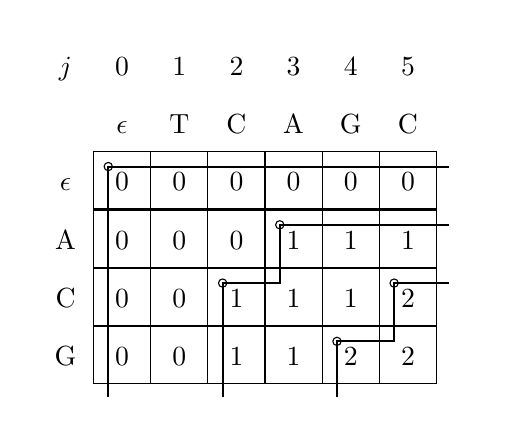
\begin{tikzpicture}[>=latex]
\matrix[mymat,anchor=west,
    box={3, 4, 5, 6}{2, 3, 4, 5, 6, 7}]
at (0,0) 
(mat1)
{ 
  $j$ & 0 & 1 & 2 & 3 & 4 & 5 \\
   & $\epsilon$ & T & C & A & G & C & \\
  $\epsilon$ & 0 & 0 & 0 & 0 & 0 & 0 &\\
  A & 0 & 0 & 0 & 1 & 1 & 1 \\
  C & 0 & 0 & 1 & 1 & 1 & 2 & \\
  G & 0 & 0 & 1 & 1 & 2 & 2 & \\
};


\begin{scope}
\coordinate(start) at([yshift=-15pt, xshift=-5pt]mat1-6-4.center);
\coordinate(t1) at([yshift=5pt, xshift=-5pt]mat1-5-4.center);
\coordinate(t2) at([yshift=5pt, xshift=-5pt]mat1-5-5.center);
\coordinate(t3) at([yshift=5pt, xshift=-5pt]mat1-4-5.center);
\coordinate(end) at([yshift=5pt, xshift=15pt]mat1-4-7.center);

\node[draw=black, circle, inner sep=0pt,minimum size=3pt] at (t1) {};
\node[draw=black, circle, inner sep=0pt,minimum size=3pt] at (t3) {};

\draw[line width=0.25mm] (start) -- (t1) -- (t2) -- (t3) -- (end);
\end{scope}

\begin{scope}
\coordinate(start) at([yshift=-15pt, xshift=-5pt]mat1-6-6.center);
\coordinate(t1) at([yshift=5pt, xshift=-5pt]mat1-6-6.center);
\coordinate(t2) at([yshift=5pt, xshift=-5pt]mat1-6-7.center);
\coordinate(t3) at([yshift=5pt, xshift=-5pt]mat1-5-7.center);
\coordinate(end) at([yshift=5pt, xshift=15pt]mat1-5-7.center);

\node[draw=black, circle, inner sep=0pt,minimum size=3pt] at (t1) {};
\node[draw=black, circle, inner sep=0pt,minimum size=3pt] at (t3) {};

\draw[line width=0.25mm] (start) -- (t1) -- (t2) -- (t3) -- (end);
\end{scope}

\begin{scope}
\coordinate(start) at([yshift=-15pt, xshift=-5pt]mat1-6-2.center);
\coordinate(t1) at([yshift=5pt, xshift=-5pt]mat1-3-2.center);
\coordinate(end) at([yshift=5pt, xshift=15pt]mat1-3-7.center);

\node[draw=black, circle, inner sep=0pt,minimum size=3pt] at (t1) {};

\draw[line width=0.25mm] (start) -- (t1) -- (end);
\end{scope}
\end{tikzpicture}

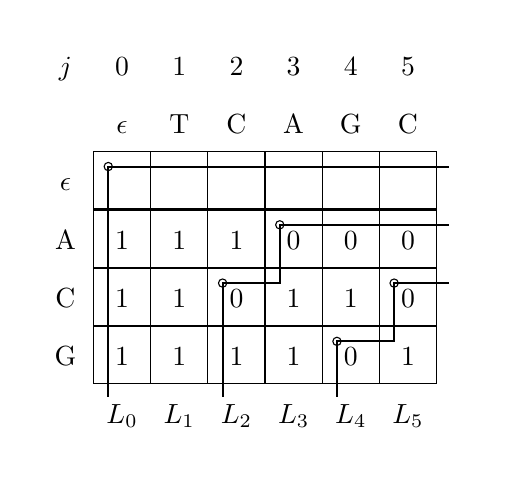
\begin{tikzpicture}[>=latex]
\matrix[mymat,anchor=west,
    box={3, 4, 5, 6}{2, 3, 4, 5, 6, 7}]
at (0,0) 
(mat1)
{ 
  $j$ & 0 & 1 & 2 & 3 & 4 & 5 \\
   & $\epsilon$ & T & C & A & G & C & \\
  $\epsilon$ &  &  &  &  &  &  &\\
  A & 1 & 1 & 1 & 0 & 0 & 0 & \\
  C & 1 & 1 & 0 & 1 & 1 & 0 & \\
  G & 1 & 1 & 1 & 1 & 0 & 1 & \\
    & $L_0$ & $L_1$ & $L_2$ & $L_3$ & $L_4$ & $L_5$ \\
};


\begin{scope}
\coordinate(start) at([yshift=-15pt, xshift=-5pt]mat1-6-4.center);
\coordinate(t1) at([yshift=5pt, xshift=-5pt]mat1-5-4.center);
\coordinate(t2) at([yshift=5pt, xshift=-5pt]mat1-5-5.center);
\coordinate(t3) at([yshift=5pt, xshift=-5pt]mat1-4-5.center);
\coordinate(end) at([yshift=5pt, xshift=15pt]mat1-4-7.center);

\node[draw=black, circle, inner sep=0pt,minimum size=3pt] at (t1) {};
\node[draw=black, circle, inner sep=0pt,minimum size=3pt] at (t3) {};

\draw[line width=0.25mm] (start) -- (t1) -- (t2) -- (t3) -- (end);
\end{scope}

\begin{scope}
\coordinate(start) at([yshift=-15pt, xshift=-5pt]mat1-6-6.center);
\coordinate(t1) at([yshift=5pt, xshift=-5pt]mat1-6-6.center);
\coordinate(t2) at([yshift=5pt, xshift=-5pt]mat1-6-7.center);
\coordinate(t3) at([yshift=5pt, xshift=-5pt]mat1-5-7.center);
\coordinate(end) at([yshift=5pt, xshift=15pt]mat1-5-7.center);

\node[draw=black, circle, inner sep=0pt,minimum size=3pt] at (t1) {};
\node[draw=black, circle, inner sep=0pt,minimum size=3pt] at (t3) {};

\draw[line width=0.25mm] (start) -- (t1) -- (t2) -- (t3) -- (end);
\end{scope}

\begin{scope}
\coordinate(start) at([yshift=-15pt, xshift=-5pt]mat1-6-2.center);
\coordinate(t1) at([yshift=5pt, xshift=-5pt]mat1-3-2.center);
\coordinate(end) at([yshift=5pt, xshift=15pt]mat1-3-7.center);

\node[draw=black, circle, inner sep=0pt,minimum size=3pt] at (t1) {};

\draw[line width=0.25mm] (start) -- (t1) -- (end);
\end{scope}
\end{tikzpicture}


\end{document}